\section{CityScope Grasbrook}\label{sec:grasbrook}

{
    \subsection{Introduction}
    {
        CityScope Grasbrook was commissioned in 2019 by the the City of Hamburg and the HafenCity Company, as part of a unique tender format for a new residential and business district in the Grasbrook, Hamburg, Germany\footnote{CityScope Grasbrook was born out of a cooperation of three institutional partners: (i) HafenCity Hamburg GmbH is a city-owned urban development agency mandated to develop large-scale projects in the city of Hamburg \cite{cgha19, br18}; (ii) the Digital City Science Lab at HafenCity University HCU; and (iii) the MIT CityScope team.}. The Grasbrook project provided a real-world opportunity to develop and test the idea of the unified and open-ended CityScope architecture (see Section \eqref{sec:cityscope_architecture}). CityScope Grasbrook is a digital online tool and participatory process, that provides algorithmic analysis and predictive simulation for early-stage urban-design proposals in a design competition stage. Specifically, the system supports the decision-making of two user groups: (i) City planners, architects, or designers, in the process of developing urban-designs proposals, and (ii) Competition juries when evaluating said proposals. The system provides instant assessment of environmental and spatial impact, such as noise propagation, pedestrian accessibility, or storm-water flooding; When evaluated, CityScope Grasbrook modules were shown to be comparable or better than experts' analysis of the same metrics.



        \begin{figure}[!htb]
            \begin{center}
                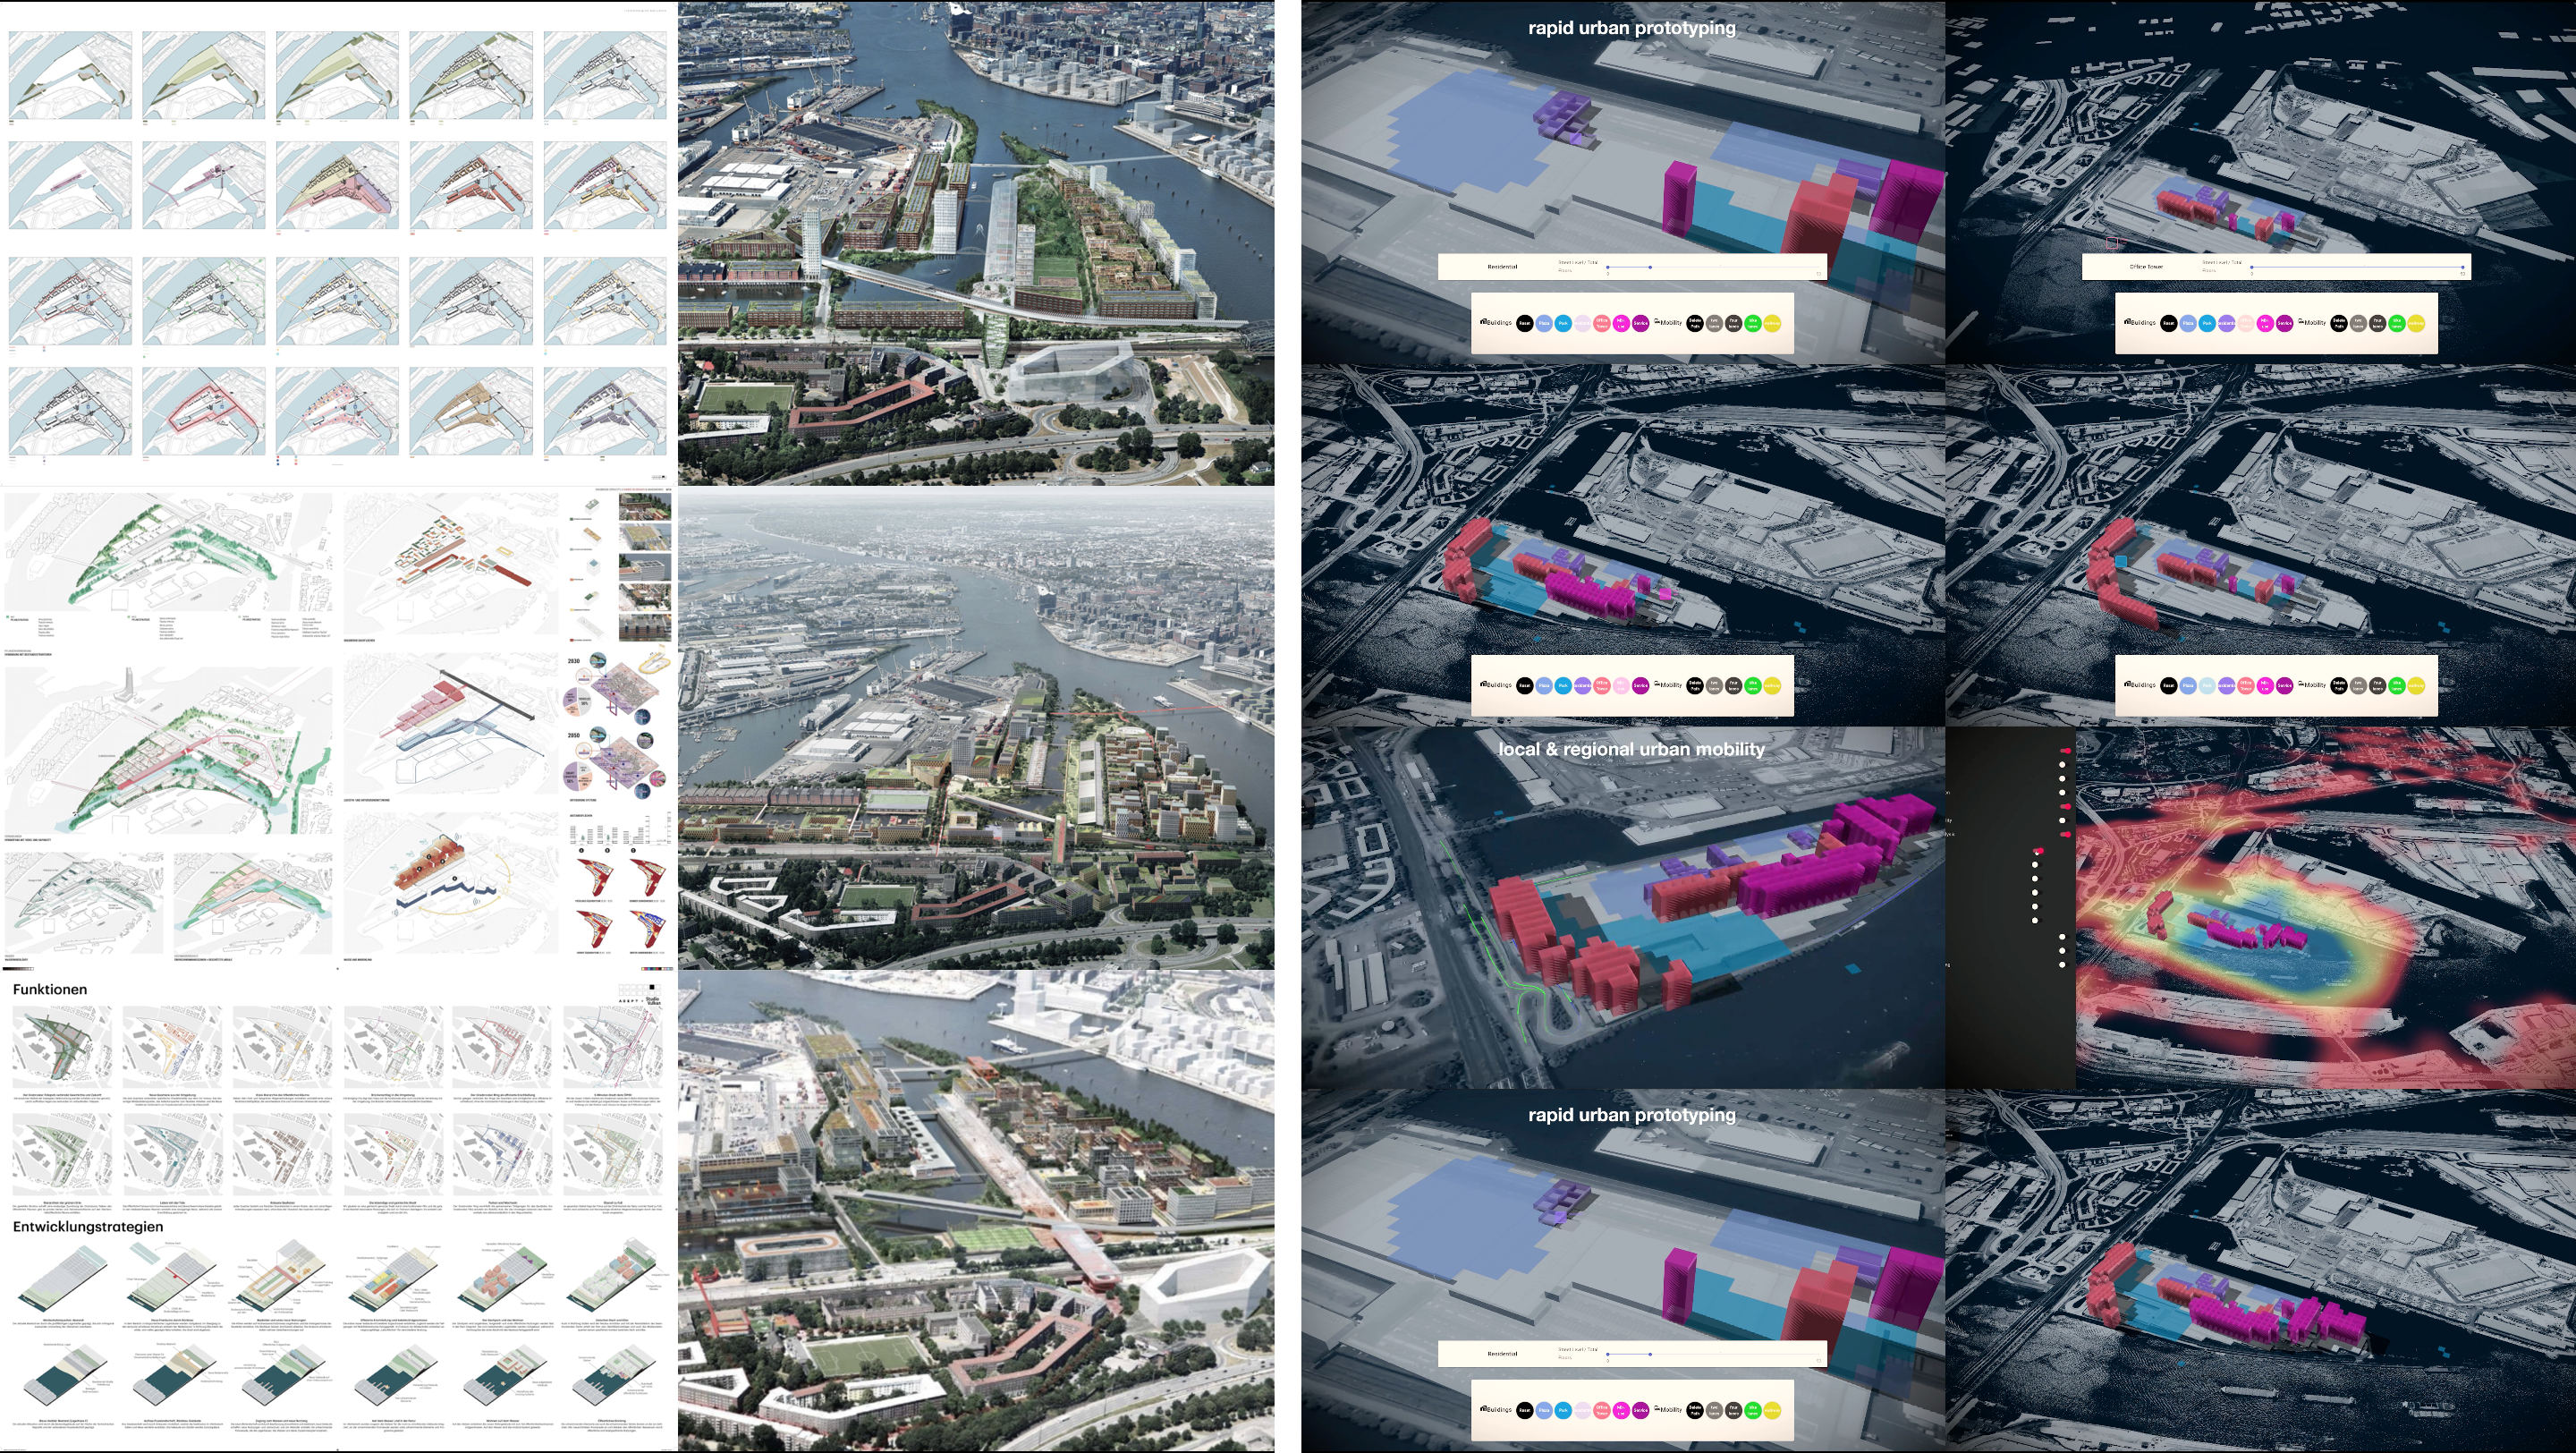
\includegraphics[width=1\textwidth]{chapters/transformation/grasbrook/figures/grsbrk5.png}
            \end{center}
            \caption{Competition submissions vs. CityScope interface. Similar to other architectural and design competitions, the Grasbrook's brief specify certain requirements for each design submission. Nevertheless, `creative freedom' and lack of a strict submission format makes it hard to properly evaluate the performance metrics of each proposal. The CityScope interface, on the other hand, is designed for an `apples-to-apples' comparisons, where the user can observe, evaluate, and correct the results of different submissions in one framework.}
            \label{fig:grasbrook_competition_vs_cs}
        \end{figure}

        \subsubsection{Motivation}
        {
            Urban development projects evolve through complex and lengthy processes: From project initiation, via public deliberation and tendering, onto the physical execution of architectural designs. In all of these stages, a multitude of stakeholders, functional requirements, and criteria must to be well coordinated \cite{alexander1990planning}. Within this process, the results of urban-design competitions play a crucial role, as their procedures and outcomes can strongly determine the shape and quality of future urban environments.
            \newline
            In this context, CityScope Grasbrook addresses two use-cases: (i) \textit{During the Design Process:} CityScope is used by design teams in the earliest phases of schematic design (SD), in which crude proposals are drafted to outline functional and spatial features of the area. In this case, the system was designed to rapidly deliver information on the effects of their drafts, to estimate their overall qualitative performance, and to optimize their spatial layout and functional programs. For example, CityScope may instantly provide answers to questions like: \textit{``How does the placement of a certain building influences the propagation of traffic noise in the area?''}
            \newline
            (ii) \textit{During Jury Review:} Here, CityScope is used later in the competition process, when expert juries assess submissions to conclude the winning entry. At this stage, CityScope helps the jurors to evaluate the submissions, to check their compliance with key criteria, and to judge the different proposals on the basis of objective performance indicators. The comparison of design proposals by way of algorithmic analysis benefits an unbiased and transparent assessment process, and can also eases the task of assessing inconsistent or non-standardized submission formats\footnote{Especially in early design phases, these deliverables could vary dramatically, from mix-media and physical models, to perspective drawings and text descriptions \cite{ben-joseph2001}.}.
        }
    }

    \begin{figure}[!htb]
        \begin{center}
            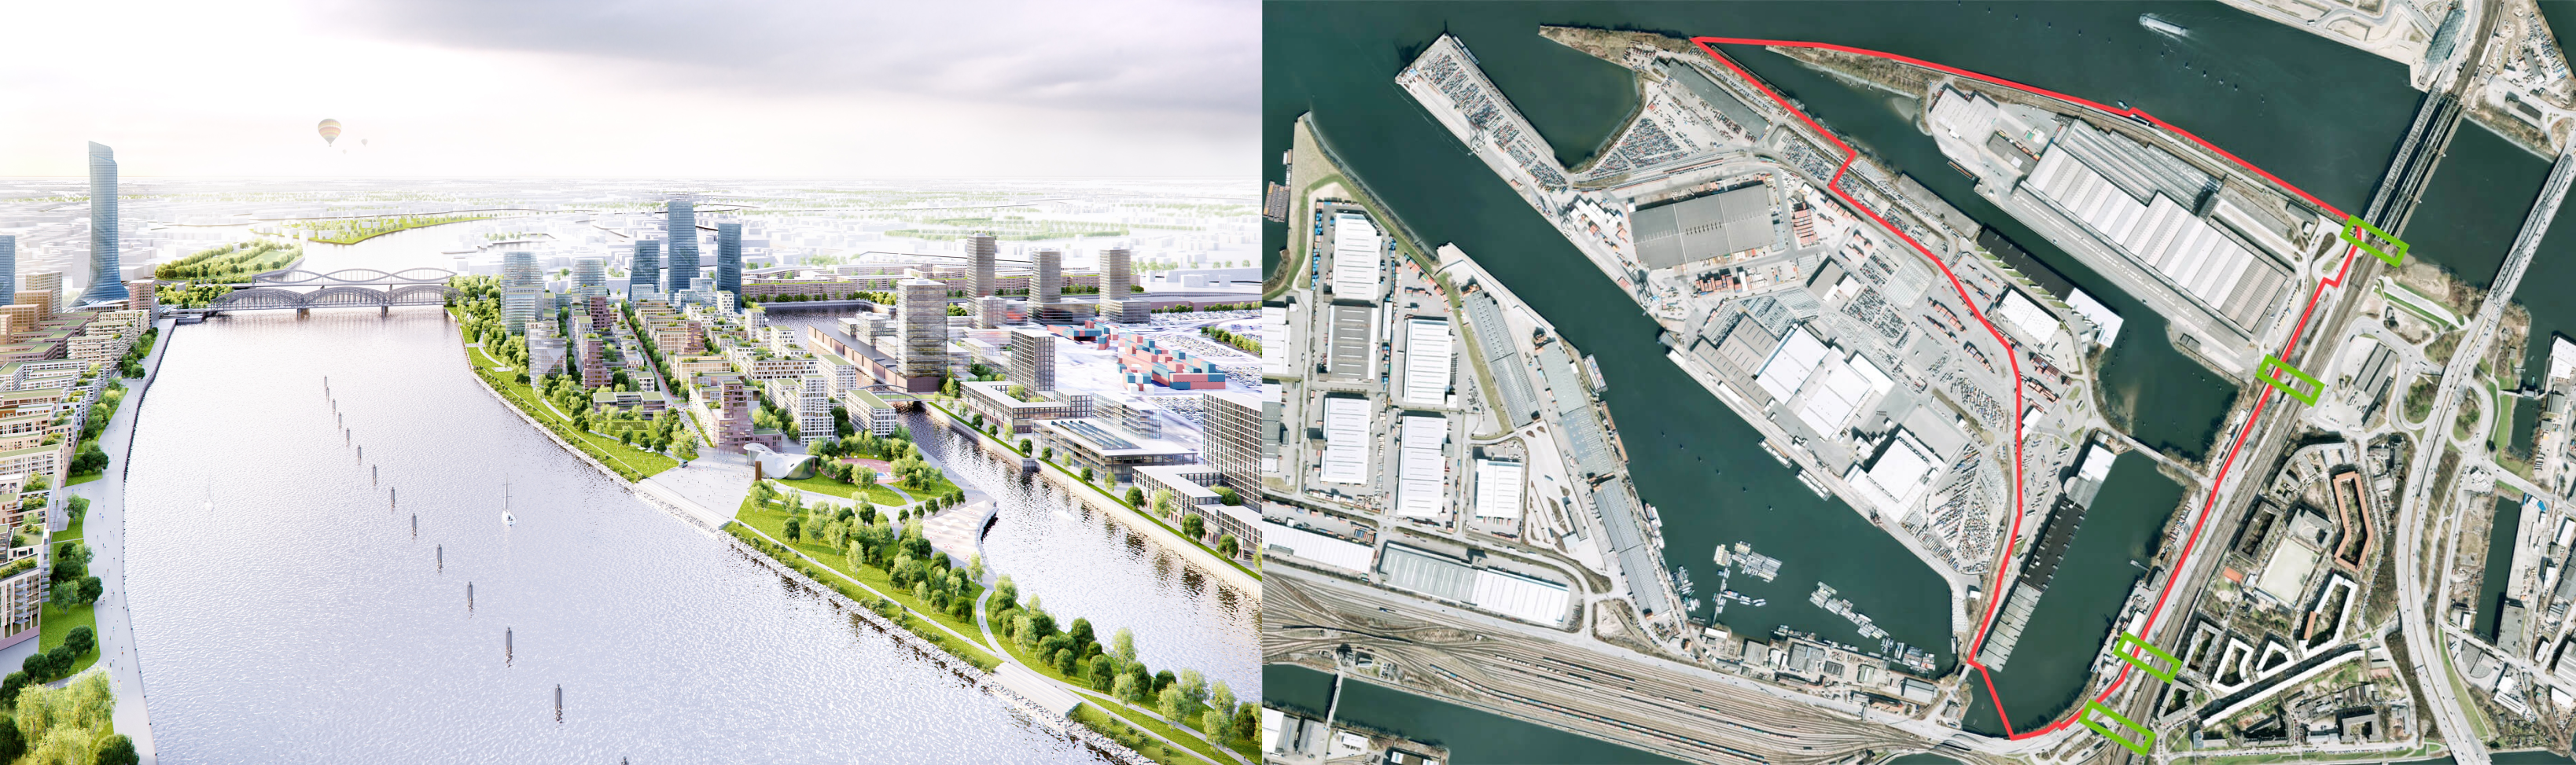
\includegraphics[width=1\textwidth]{chapters/transformation/grasbrook/figures/grsbrk1.png}
        \end{center}
        \caption{Grasbrook site (right) showing the active harbor section in the south-west, and the Veddel neighborhood to the east. (left) Previous design studies for Grasbrook, by Hosoya Schaefer Architects, Zurich.}
        \label{fig:grasbrook_site}
    \end{figure}

    \subsection{`Competitive Dialogue'}
    {
        A ``Competitive Dialogue'' is a bidding framework designed for complex urban development projects \cite{hpg15}. For the Grasbrook site, the bidding was announced EU-wide, and twelve teams (six urban-design and six landscape-design offices) were invited\footnote{The HafenCity Hamburg GmbH who published and managed the tender, acted as an intermediary between ministries, citizens, experts and design teams in order to supply data and feedback for the iterative improvement of their design schemes.}. In phase one, the teams worked independently within their professional domains; After the conceptual phase, six offices were submerged into three mixed teams, who were asked to propose an holistic landscape and urban-design solution. After the second phase, one winning team was selected by a high-level jury in April 2020.
    }



    \subsection{Platform Design}

    {
        CityScope Grasbrook utilized the unified CityScope architecture (see Section \eqref{sec:cityscope_architecture}) as a baseline for the development of a custom set of analysis modules and feedback features. This system design was well suited for the Grasbrook use-case, since it could host a myriad of analytic tools, whose interconnection enables an algorithmic analysis of complex cause-and-effect chains created by urban-design interventions.

        \begin{figure}[!htb]
            \begin{center}
                \includegraphics[width=1\textwidth]{chapters/transformation/grasbrook/figures/grsbrk3.jpg}
            \end{center}
            \caption{Grasbrook CityScope System Architecture: Following the CityScope Schema and system design, Grasbrook adapted a parallel data flow between the different components (see Section \eqref{sec:cityscope_architecture}).}
            \label{fig:grasbrook_architecture}
        \end{figure}

        \textbf{Modular Architecture:} CityScope Grasbrook was designed as an online platform first, which could later be extended to TUI and other interfaces as needed. The overall architecture consists of a frontend UI and a set of various backend analysis modules, all of which are connected via cityIO (see \eqref{subsec:csarch-cityio}). With this structure, different software applications for the analysis of specific urban KPIs (i.e. noise propagation, storm-water runoff, pedestrian accessibility) or target indicators (Gross Floor Area, FAR) can be easily plugged-in yet independently developed by different teams.
        \newline
        \textbf{Security Features:} Specific to the Grasbrook case-study, secure storage of the competitors' project data was required. Simultaneous user-access to the CityScope platform, as well as backend data management, had to comply with security and confidentiality standards. Considering legal controversies that sometimes emerge in the aftermath of design competitions, the CityScope team implemented several data security and safety measures: secure user authentications, individual usernames and passwords for each participant, access monitoring, real-time system logging and analytics. These features were implemented in the frontend UI, and the backend cityIO server.


        \begin{figure}[!htb]
            \begin{center}
                \includegraphics[width=1\textwidth]{chapters/transformation/grasbrook/figures/grsbrk4.jpg}
            \end{center}
            \caption{Translation of design submissions into CityScope grid. When complex shapes are presented, or negative volumes calculation is need for GFA calculations, the grid approach might be less accurate.}
            \label{fig:grasbrook_pixel_translation}
        \end{figure}
    }


    \textbf{Interaction Design:} As with other CityScope projects, site and intervention data is translated into the form of a grid and the CityScope Schema \eqref{sec:cityscope_architecture}, enabling faster modules' calculations and real-time user interaction. This transformation is performed by transferring the morphology of the site into a 2D raster\footnote{in the Grasbrook case, the grid was of 16x16 meters and four meters for ground level, three meters on upper levels}. Each grid cell hold information about its usage (built or unbuilt) along with its core functions (residential, commercial, educational, promenade, street, park, etc.). In the context of the Grasbrook competition, the matrix reflects (i) A standard measure for minimum street width according to heat flow and pollutant dispersion metrics \cite{yc18}; (ii) A building depth allowing natural cross-ventilation and daylight penetration \cite{mn19}; (iii) A suitable level of detail for visualization, allowing intuitive and real-time feedback for user interaction; and (iv) A documented metric for other similar cases of computational urban simulations.


    \subsection{Analytic Modules}

    {
        HafenCity Hamburg GmbH prioritized four types of analytic modules: noise propagation, storm-water runoff, walkability, and gross floor area (GFA). These modules were deemed as key in the decision-making process of the competition, as they commonly hard to infer from the design submission themselves. The following is a description of each module, and an evaluation of its performance and usability.

        \begin{figure}[!htb]
            \begin{center}
                \includegraphics[width=1\textwidth]{chapters/transformation/grasbrook/figures/grsbrk2.jpg}
            \end{center}
            \caption{Goals of each of the CityScope modules used in Grasbrook. As with other CityScope projects, each module should aim to answer a specific question. For CityScope users, the overlapping of different modules' responses creates a deeper understanding of the design tradeoffs, for example: `Would this intervention promote both easier access AND better water management?'}
            \label{fig:grasbrook_modlues_questions}
        \end{figure}


        \subsubsection{Modules Accuracy}
        {
            This project was a first opportunity to test the CityScope modular architecture in real-world use-case. This required a high level assessment of modules' quality and reliability, for both the design teams as well as the jurors. In communications to the design teams, trade-offs between usability, speed of interaction, and quality of assessment were highlighted.
            While higher accuracy and reliability could only come from expert reports and industry standard, these tend to be costly, take substantially longer time to produce, and would not be as iterative as the CityScope layouts. Since CityScope pixelates the raster of the design space, calculating the level of accuracy was done by comparing modules' output with rasterized results of analysis preformed by external committee of experts\footnote{The introduction of CityScope to the Grasbrook tender had to comply with organizational and legal constraints. Due to the academic nature of the project, it was necessary to distinguish the features and outputs of the CityScope solution from those of accredited expert tools. When introduced to the competition teams, the aim and character of the scientific experiment were communicated, and it was maintained that the solution would not deliver legally binding output or assessments, but rather provide additional support for the decision-making process.}.
        }



        \begin{figure}[!h]
            \begin{center}
                \includegraphics[width=.7\textwidth]{chapters/transformation/grasbrook/figures/grsbrk0.png}

            \end{center}
            \caption{
                Analytic modules developed for the Grasbrook competition (From the top):
                (i) CityScope noise analysis result compared to experts' analysis for the winning competition entry; (ii) CityScope results of runoff coefficients. Estimated annual runoff volumes m\textsuperscript{3} by surface type. Upper Right: Qualitative evaluation used to assess schematic map submissions; (iii) Walkability calculations results for user type `adult' and `cultural institutions'. Areas in green show the travel distance below the threshold of a five-minute walk. Upper Right: Qualitative evaluation method used to assess submission materials, including schematic maps, explanatory sketches, and pictograms.
            }
            \label{fig:grasbrook_results}
        \end{figure}

        \subsubsection{Noise Module}
        {
            Noise emission is a key concern in urban-design and city-planning. Grasbrook site is situated near major transit arteries, highways, railways, as well as an industrial port area, making the appropriate estimation of acoustic impact, a crucial item in the evaluation of design proposals \cite{e19}. In conventional planning procedures, noise performance of design proposals is usually possible only through expert evaluation in advanced stages, sometimes years after the initial competition phase has been concluded. In contrast, the noise module developed for the Grasbrook CityScope was able to model noise propagation throughout the design area in near real-time.
            \newline
            This module considers noise emitters, such as large streets and adjacent railway lines, on the basis of predicated traffic loads. It uses software developed by the French Institute of Science and Technology for Transport, Development and Networks \cite{bgppf19}, which is based on a simplified implementation of the French standard for urban noise propagation, NMPB-08 \cite{n11}. When designers interact with the CityScope grid, the noise simulation tool extracts building footprints and calculates a 2D noise distribution map. The noise emitted by simulated traffic on streets and railways is propagated through the design area, taking into account the diffractions and reflections caused by the buildings.
            \newline
            \textbf{Evaluation and Validation:} In order to evaluate the noise module accuracy, the CityScope noise module were compared to results retrieved from an established noise modeling consultancy. Figure \eqref{fig:grasbrook_results} presents the results of the analysis of the winning competition entry performed with the CityScope tool compared to the results delivered by the external consultancy. Visually, both noise maps shows similar dispersal patterns. When rasterizing both result sets, a differential map is computed to locate and visualize the differences in estimated noise levels. This differential map indicates that the total area of noise level differences greater than 10dB are below 7.5\% of the design area, whereas 53\% of the design area show deviations of max 5db. The remaining 39.5\% of the design area shows deviations between 5 and 10 dB.
            \newline
            Studies have shown that different experts evaluating noise using different national methods create results which deviate by 10 to 15dB \cite{nw05}. In this case, a main cause for the deviation results is the different calculation methods used by the CityScope and the external consultancy, which differ in the standard metrics utilized\footnote{Simplified implementation of the French NMPB-08 standard for CityScope vs. German RLS 90 standard for road noise sources and unspecified methods for propagation calculation Consultancy}. Moreover, technical differences and input assumptions influence the definition of noise modeling accuracy, such as:
            (i) Rasterized CityScope input format leads to simplifications of the design proposal, from building footprints to a grid-based input;
            (ii) Experts added higher noise levels to context-specific locations (e.g., bridges over the Elbe River);
            (iii) French and German standards use different annotation scales for noise levels;
            (iv) CityScope delivers a composite day, evening and night index (LDEN) while the method deployed by the external consultancy indexes for daytime only.
            \newline
            As a general trend, the results delivered by the CityScope generally show lower noise levels than the ones delivered by the external consultancy. Still, a proportional behavior and distribution of the noise levels underline the applicability of the tool for real-time noise modeling.
        }


        \subsubsection{Storm-water Module}
        {
            As in many other parts of the city of Hamburg, the Grasbrook district is vulnerable to flooding caused by heavy rainfall events and sea-level rise. The HafenCity Hamburg GmbH requested a storm-water module in order to evaluate the synergies between green storm-water infrastructure, comfortable microclimatic conditions, and the functional requirements for landscape design. This module calculates the surface runoff from each cell in the CityScope grid, and combines it to an annual storm-water runoff analysis. Each cell of the grid contains data about the surface type (e.g., building, street, open-space) and each type is assigned a runoff coefficient\footnote{The runoff coefficients were adapted from Table 9 of DIN 1986-100:2016-12 \cite{e16}.}. The $m^2$ area of each cell is multiplied by the runoff coefficient and by the annual rainfall $m^3/m^2*a$.
            \newline
            \textbf{Evaluation and Validation:} Today, most experts rely on schematic blueprints or renderings to evaluate storm-water potential. These schematics often lack the information necessary to evaluate the submissions beyond a baseline qualitative assessment. CityScope storm-water module uses standardized measures of surface permeability and infiltration potential, in order to estimate cumulative annual runoff volumes. While expert analysis for water-cycles usually involves a tricolor rating system, CityScope enables a quantitative comparison of the design submissions in their entirety, while still supporting qualitative assessments.
            \newline
            Nevertheless, some spatial aspects were not consistently present in all design submissions, for example: (i) Topography within the area; (ii) Directional flows within the storm-water network, and (iii) Location and size of infrastructure, such as infiltration, retention, water treatment facilities, or neighborhood cistern. Consequently, the Grasbrook version of the storm-water module did not include these aspects, either. Already in its current form, the storm-water module can deliver a valuable quantitative comparison of the designs in regards to the ratio of green and open-space, as well as annual runoff projections from differentiated surface types.
        }

        \subsubsection{Walkability Module}
        {
            Walkability is a key parameter in the evaluation of urban districts and neighborhoods design \cite{carr1969city, krier1979urban}. Human-centred urban-design promotes the development of neighborhoods that well-function without broad usage of motorized vehicles; In order to prevent unnecessary traffic and subsequent negative environmental impacts, basic amenities and socio-spatial infrastructure need to be accessible to all local residents within a minimal walking distance \cite{banerjee2011companion}. In order to identify the distribution of services and amenities during early urban-design processes, an analytic module was devised to calculate the 5-minute walkshed of a subset of amenities, such as educational, cultural or retail. The tool implements a standardized isochrone calculation using the walkable street network, a common method utilized in walkability and accessibility research \cite{dp20, dwp17}.
            \newline
            \textbf{Evaluation and Validation:} While the expert analysis was based on a qualitative evaluation of the pedestrian network, CityScope numerically calculated the accessibility based on the street network morphology in the proposal. Specifically, the module calculated accessibility to-and-from different amenity types, using three main trip profiles: adult, child, and wheelchair user. Each of the walking profiles includes an average speed and a list of surfaces through which they can traverse comfortably; For example, wheelchair users might not be able to pass through streetscape involving stairs or steep slopes. The walkability calculation for each amenity type, and each walking profile, is performed using a flood-fill calculation performed by Dijkstra's shortest path algorithm on the CityScope grids \cite{eldg14}. The CityScope walkability module enables quantitative analysis of accessibility, complementing the mostly qualitative interpretation provided by the mobility and transportation experts.
        }

        \subsubsection{GFA Module}
        {
            A common indicator for the economic and spatial feasibility of urban-design is the Gross Floor Area (GFA) \cite{fcc18}. Balancing between economic profitability (production of marketable real-estate) and spatial quality (openness, view, visibility), is a key in urban-design processes. The definition of GFA do not only affect physical parameters (e.g., distribution of light and shadow) but also local logistics and supplies, as well as the provisioning of social infrastructure (e.g., day-care or medical facilities). The CityScope GFA module calculates the aggregated GFA in square meters in respect to the classification of building-use defined in the competition brief.
            \newline
            \textbf{Evaluation and Validation:} Given the simplification imposed by CityScope grid rasterization (see Section \eqref{subsec:types_system}), the accuracy of this module depends on the granularity of the design submission, and their adherence to parallel lines, or right angles. Naturally, freeform-designs achieve lower accuracy in GFA analysis than designs based on rectangular blocks, due to deviations in the calculated floor area. In order to determine the accuracy of the module, calculations were compared with expert evaluation reports which include a cross-check of designed volumes against the definitions made by the competition brief \cite{e19}. The main land-use categories, `Commercial' and `Residential,' correspond closely with the same use types in the competition brief, whereas the CityScope category `Other' roughly translates to `Special use,' which includes cultural, educational, and sports usages.
            \newline
            Differences in type classification between CityScope and the competition brief, the transformation of the designs to the CityScope grid, and subjective data entry, contributed to misalignment in GFA module results, compared to experts evaluation. In 7 of 8 cases, the absolute difference ranged from 1\% to 27\%, with an average of absolute difference of 14\%. For one competition entry, the absolute difference was 170\% for `Other' due to the user's interpretation of non-standard mixed use types as `Other' rather than primarily `Residential' or `Commercial'. In future use-cases, a GFA module should be designed in a more flexible way, so that it could match GFA requirements of a competition brief.
        }
    }

    \subsection{Discussion}
    {
        The Grasbrook project was the first opportunity to involve CityScope system, including frontend, modules, cityIO, and other components, in a real-world design competition process.
        CityScope Grasbrook was implemented for two different use-cases: (i) Designers and planners developing design proposals during the competition, and (ii) Competition juries evaluation of these design proposals. This section evaluates the usage of CityScope for each of the two use-cases.

        \subsubsection{Strengths}
        {
            The time and cost of obtaining expert analysis is a major obstacle in the creation of feasible, sustainable and well-balanced urban-design proposals. CityScope compensates this deficit by delivering data-driven and real-time results during the design process. Moreover, CityScope architecture promotes a single data input (CityScope Grid, see Section \eqref{sec:cityscope_architecture}) which is shared across the different analytic modules. This structure avoids inputting design schemes into separated software applications, or carry out time-consuming data transfer and reformatting.
            \newline
            Additionally, CityScope provides a standardized assessment of both spatial, environmental, and social qualities of urban-design proposals. It enables an objective assessment of completely different designs, which is particularly useful when evaluating several proposals under the same set of criteria. Simplified interaction and standard visualization make the comparison of proposals substantially easier, for both the design juries and designers themselves. CityScope's standardized data format, and open-source modules provide transparency in the process of analysis and assessment, and allow technical consensus amongst domain-experts.
        }

        \subsubsection{Weaknesses}

        {
            The accuracy of the analytic modules remains a scientific and methodological challenge. Designers, juries, developers, or investors depend on clear indications and relative reliability compared to well-established methods of evaluation. While validation was preformed for the noise and rainwater modules, the discrepancy of scientific models, methodology, and data schemes, challenges an in-depth validation and refinement of other modules.
            \newline
            Even though one single data structure (CityScope Grid) can be more time efficient compared to several data inputs and separated applications, the current tool required that the designs would be manually uploaded. This was accomplished by importing multiple layers of geospatial information (e.g., existing buildings, site restrictions), as well as rasters of the first round designs, to allow users to translate them into CityScope grids. To make the input and translation process easier, users expressed interest to import data formats common for their preferred design software or competition submission files (e.g., DWG, RVT, IFC). In the future, such data conversion pipeline could be added to CityScope for automatic CAD and BIM data conversion.
        }

        \subsubsection{Opportunities}
        {
            A key benefit of CityScope is its capacity to run different types of analysis at the same time. In this respect, it has greater analytic power than evaluations which only consider one dimension at a time. By changing the layout of a plot or a building in one specific setting, impacts on many different other KPIs and metrics can be observed. By cross-connecting the various analytic modules, new inputs will simultaneously change and update other performance layers.
            \newline
            Validated CityScope modules and open-source development, can ensure that the evaluation of design proposals will not be delivered as rigid `black-box' solutions. Open-source development makes non-generic modules (such as site-specific analysis) easily adaptable to other future scenarios, and allows for better validation by the scientific community. As a digital online tool, CityScope has the potential to facilitate communication and dialogue with larger stakeholders groups, neighborhood communities, local initiatives, or academia.
        }

        \subsubsection{Threats}
        {
            The introduction of new processes and technologies can be accompanied by scepticism and rejection from its target audience. Designers tend to have well-established workflows, especially in the stressful context of design competition projects, where they rely on conceptual and technical traditions adopted over years. Similarly, jurors might not welcome the appearance of new decision-support systems: discrepancies and conflicts between expert judgement and algorithmic analysis may occur, and might be considered a disruption of established power-structures and political dominance. It is therefore critical to properly position CityScope-like tools as decision-support systems, not a replacement for experts and community discussion.
        }

    }

    \subsection{Conclusion}
    {
        CityScope Grasbrook was an initial attempt to \textit{`reinvent the competition'}, by offering an open-ended digital platform for design analysis and evaluation. This project has demonstrated its applicability for high-stake international urban-design competition, by effectively supporting the decision making of (i) Designers and planners in the process of developing sustainable urban-designs proposals, and (ii) Competition juries mandated for the evaluation of the final proposals. To both, CityScope provided instant assessment and analytic evidence via multiple key metrics.
    }
}






















